% ==========================================================================
%  FlairSim — Documentation technique complète
%  Simulateur de drone sur imagerie aérienne FLAIR-HUB
%  Fil rouge — Mastère Spécialisé Big Data / IA, Télécom Paris
% ==========================================================================
\documentclass[a4paper, 11pt, french]{article}

% ---- packages fondamentaux ----
\usepackage[utf8]{inputenc}
\usepackage[T1]{fontenc}
\usepackage{babel}
\usepackage{lmodern}
\usepackage{microtype}

% ---- mise en page ----
\usepackage[margin=2.2cm]{geometry}
\usepackage{parskip}
\usepackage{fancyhdr}

% ---- code, liens, couleurs ----
\usepackage{listings}
\usepackage{xcolor}
\usepackage[colorlinks=true, linkcolor=blue!60!black, urlcolor=blue!60!black,
            citecolor=blue!60!black, hypertexnames=false]{hyperref}

% ---- tableaux, figures, maths ----
\usepackage{booktabs}
\usepackage{array}
\usepackage{longtable}
\usepackage{graphicx}
\usepackage{amsmath}
\usepackage{float}
\usepackage{caption}
\usepackage{subcaption}

% ---- diagrammes TikZ ----
\usepackage{tikz}
\usetikzlibrary{arrows, positioning, fit, backgrounds, calc, shapes.geometric,
                 decorations.pathreplacing, shadows}

% ---- code listing style ----
\definecolor{codebg}{RGB}{248,248,248}
\definecolor{codeframe}{RGB}{200,200,200}
\definecolor{codecomment}{RGB}{0,128,0}
\definecolor{codestring}{RGB}{163,21,21}
\definecolor{codekeyword}{RGB}{0,0,180}

% ---- architecture diagram colors ----
\definecolor{orchcolor}{RGB}{70,130,180}    % steel blue
\definecolor{simcolor}{RGB}{60,179,113}     % medium sea green
\definecolor{corecolor}{RGB}{255,165,0}     % orange
\definecolor{dronecolor}{RGB}{147,112,219}  % medium purple
\definecolor{mapcolor}{RGB}{205,92,92}      % indian red
\definecolor{webcolor}{RGB}{100,149,237}    % cornflower blue
\definecolor{viewercolor}{RGB}{144,238,144} % light green
\definecolor{datacolor}{RGB}{255,215,0}     % gold
\definecolor{clientcolor}{RGB}{255,182,193} % light pink
\definecolor{ssecolor}{RGB}{255,127,80}     % coral

\lstset{
  language=Python,
  basicstyle=\ttfamily\small,
  backgroundcolor=\color{codebg},
  frame=single,
  rulecolor=\color{codeframe},
  commentstyle=\color{codecomment}\itshape,
  stringstyle=\color{codestring},
  keywordstyle=\color{codekeyword}\bfseries,
  showstringspaces=false,
  breaklines=true,
  breakatwhitespace=true,
  tabsize=4,
  captionpos=b,
  aboveskip=8pt,
  belowskip=8pt,
}

\lstdefinestyle{bash}{
  language=bash,
  morekeywords={uv,curl,pytest,ruff,flairsim},
  deletekeywords={test},
}

\lstdefinestyle{json}{
  language={},
  morestring=[b]",
  literate=
    *{:}{{{\color{codekeyword}:}}}{1}
    {,}{{{\color{codekeyword},}}}{1}
    {\{}{{{\color{codekeyword}\{}}}{1}
    {\}}{{{\color{codekeyword}\}}}}{1}
    {[}{{{\color{codekeyword}[}}}{1}
    {]}{{{\color{codekeyword}]}}}{1},
}

\lstdefinestyle{yaml}{
  language={},
  morestring=[b]",
  morestring=[b]',
  morecomment=[l]{\#},
  morekeywords={scenario_id,name,description,dataset,data_dir,domain,roi,
                modalities,source,start,target,radius,max_steps,prompt,
                system,user_template,environment,difficulty,x,y,z},
  keywordstyle=\color{codekeyword},
  commentstyle=\color{codecomment}\itshape,
  stringstyle=\color{codestring},
}

% ---- en-têtes / pieds de page ----
\pagestyle{fancy}
\fancyhf{}
\fancyhead[L]{\small\textsc{FlairSim --- Documentation technique}}
\fancyhead[R]{\small Télécom Paris}
\fancyfoot[C]{\small\thepage}
\renewcommand{\headrulewidth}{0.4pt}
\renewcommand{\footrulewidth}{0pt}

% ---- commandes utilitaires ----
\newcommand{\code}[1]{\texttt{#1}}
\newcommand{\flairsim}{\textsc{FlairSim}}
\newcommand{\apiendpoint}[2]{\texorpdfstring{\texttt{#1}~\texttt{#2}}{#1 #2}}
\newcommand{\httpmethod}[1]{\texttt{\textbf{#1}}}

% ---- tikz styles ----
\tikzset{
  component/.style={draw, rounded corners=4pt, minimum width=3cm,
                    minimum height=1cm, font=\small\sffamily,
                    fill=#1!15, draw=#1!60, thick, align=center},
  component/.default=orchcolor,
  arrow/.style={-stealth', thick, draw=gray!70},
  darrow/.style={stealth'-stealth', thick, draw=gray!70},
  label/.style={font=\scriptsize\sffamily, text=gray!80},
  seqactor/.style={rectangle, draw, fill=#1!15, minimum width=2cm,
                   minimum height=0.7cm, font=\small\sffamily, rounded corners=2pt,
                   align=center},
  seqactor/.default=orchcolor,
  seqmsg/.style={-stealth', thick},
  seqret/.style={-stealth', thick, dashed},
  seqbox/.style={draw=gray!40, fill=gray!5, rounded corners=2pt},
}

% ==========================================================================
\begin{document}

% ---- page de titre ----
\hypersetup{pageanchor=false}
\begin{titlepage}
\centering
\vspace*{2cm}
{\Huge\bfseries FlairSim\par}
\vspace{0.4cm}
{\Large Simulateur de drone sur imagerie aérienne FLAIR-HUB\par}
\vspace{1.5cm}
{\large\bfseries Documentation technique complète\par}
\vspace{0.3cm}
{\normalsize Architecture, API, diagrammes de séquence\par}
\vspace{2cm}
{\normalsize
Fil rouge --- Mastère Spécialisé Big Data / Intelligence Artificielle\\
Télécom Paris\par}
\vspace{1cm}
{\normalsize \today\par}
\vfill
{\footnotesize
Basé sur FLAIR-HUB~\cite{flairhub} et FlySearch~\cite{flysearch}\par}
\end{titlepage}

\setcounter{page}{1}
\hypersetup{pageanchor=true}

% ---- table des matières ----
\tableofcontents
\newpage

% ======================================================================
\section{Introduction}
% ======================================================================

\flairsim{} est un simulateur de drone léger, écrit entièrement en
Python, conçu pour survoler de l'imagerie aérienne réelle issue du
jeu de données \textbf{FLAIR-HUB}~\cite{flairhub} publié par l'IGN.

Le système expose deux niveaux d'interface~:
\begin{enumerate}
  \item Un \textbf{serveur simulateur} (\code{flairsim-server}) avec
        API HTTP REST + SSE pour le pilotage direct par un agent.
  \item Un \textbf{orchestrateur web} (\code{flairsim-web}) qui gère
        des sessions isolées, sert une SPA navigateur, et persiste les
        résultats dans un leaderboard SQLite.
\end{enumerate}

% ======================================================================
\section{Architecture haut niveau}
\label{sec:archi-haut}
% ======================================================================

\subsection{Vue d'ensemble du système}

\begin{figure}[H]
\centering
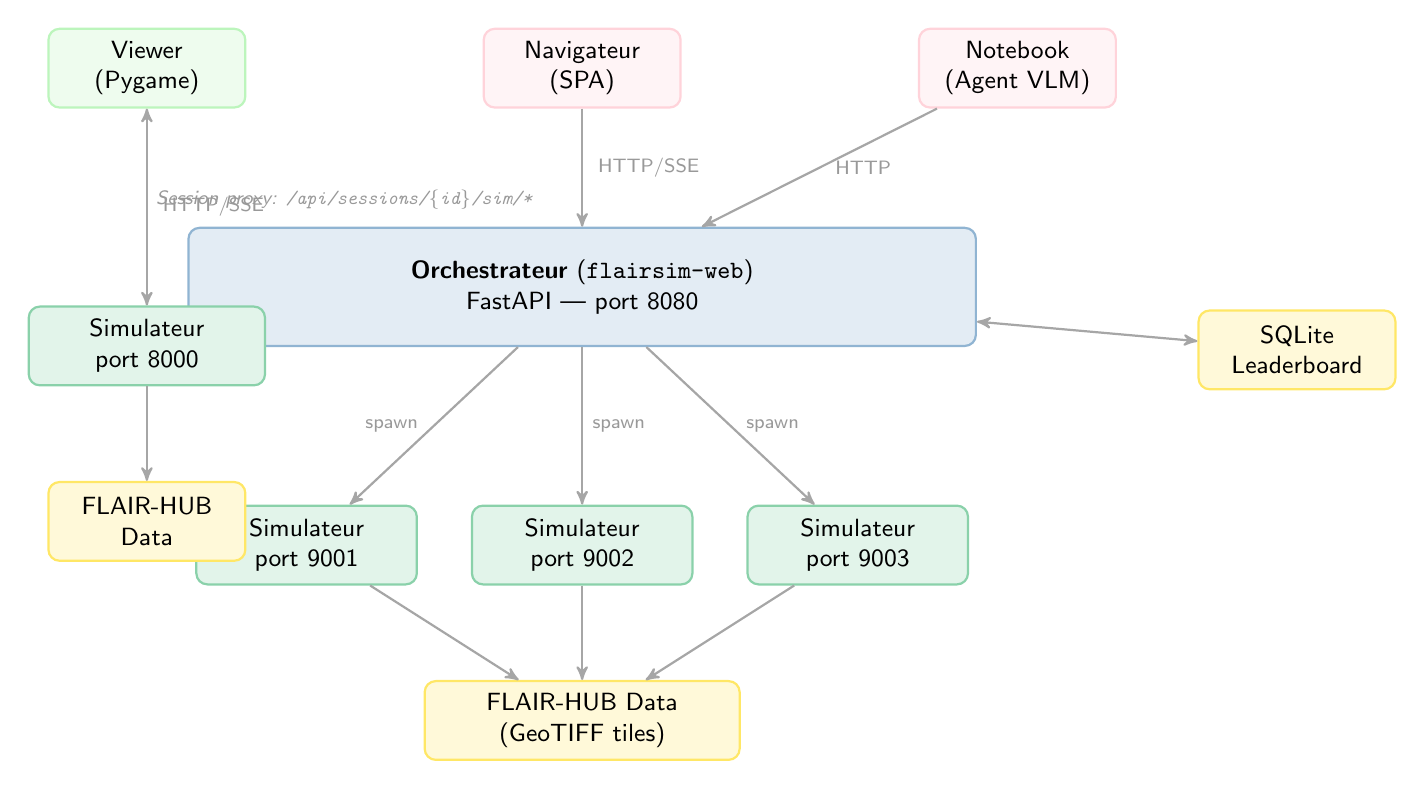
\begin{tikzpicture}[node distance=1.2cm and 2cm]

  % --- Clients ---
  \node[component=clientcolor, minimum width=2.5cm]
    (browser) {Navigateur\\(SPA)};
  \node[component=clientcolor, minimum width=2.5cm, right=3cm of browser]
    (notebook) {Notebook\\(Agent VLM)};
  \node[component=viewercolor, minimum width=2.5cm, left=3cm of browser]
    (viewer) {Viewer\\(Pygame)};

  % --- Orchestrator ---
  \node[component=orchcolor, minimum width=10cm, minimum height=1.5cm,
        below=1.5cm of browser]
    (orch) {\textbf{Orchestrateur} (\code{flairsim-web})\\
            FastAPI --- port 8080};

  % --- Simulators ---
  \node[component=simcolor, minimum width=2.8cm, below=2cm of orch,
        xshift=-3.5cm]
    (sim1) {Simulateur\\port 9001};
  \node[component=simcolor, minimum width=2.8cm, below=2cm of orch]
    (sim2) {Simulateur\\port 9002};
  \node[component=simcolor, minimum width=2.8cm, below=2cm of orch,
        xshift=3.5cm]
    (sim3) {Simulateur\\port 9003};

  % --- Direct simulator ---
  \node[component=simcolor, minimum width=3cm, below=2.5cm of viewer]
    (simdirect) {Simulateur\\port 8000};

  % --- Data ---
  \node[component=datacolor, minimum width=4cm, below=1.2cm of sim2]
    (data) {FLAIR-HUB Data\\(GeoTIFF tiles)};

  \node[component=datacolor, minimum width=2.5cm, below=1.2cm of simdirect]
    (datadirect) {FLAIR-HUB\\Data};

  % --- Leaderboard ---
  \node[component=datacolor, minimum width=2.5cm, right=0.8cm of orch,
        yshift=-0.8cm, xshift=2cm]
    (lb) {SQLite\\Leaderboard};

  % --- Arrows ---
  \draw[arrow] (browser) -- node[label, right, xshift=2pt] {HTTP/SSE} (orch);
  \draw[arrow] (notebook) -- node[label, right, xshift=2pt] {HTTP} (orch);
  \draw[arrow] (orch) -- node[label, left, xshift=-2pt] {spawn} (sim1);
  \draw[arrow] (orch) -- node[label, right] {spawn} (sim2);
  \draw[arrow] (orch) -- node[label, right, xshift=2pt] {spawn} (sim3);
  \draw[darrow] (orch) -- (lb);

  \draw[arrow] (sim1) -- (data);
  \draw[arrow] (sim2) -- (data);
  \draw[arrow] (sim3) -- (data);

  \draw[darrow] (viewer) -- node[label, right, xshift=2pt] {HTTP/SSE} (simdirect);
  \draw[arrow] (simdirect) -- (datadirect);

  % --- Labels ---
  \node[label, above=0.1cm of orch, xshift=-3cm]
    {\textit{Session proxy: \code{/api/sessions/\{id\}/sim/*}}};

\end{tikzpicture}
\caption{Architecture deux tiers --- Orchestrateur + Simulateurs isolés}
\label{fig:archi-haut}
\end{figure}

\textbf{Principes de conception~:}
\begin{itemize}
  \item \textbf{Isolation par sous-processus}~: chaque session reçoit son
        propre processus \code{python -m flairsim.server}. Aucune
        interférence entre sessions.
  \item \textbf{Pool de ports}~: ports 9001--9099 alloués dynamiquement,
        recyclés à la destruction. Max 99 sessions concurrentes.
  \item \textbf{Proxy transparent}~: l'orchestrateur relaie toutes les
        requêtes vers le bon sous-processus via \code{httpx}.
  \item \textbf{SSE proxy}~: le flux SSE est relayé en streaming
        via \code{httpx.AsyncClient.stream()}.
  \item \textbf{Aucun code VLM sur le serveur}~: les agents tournent
        à l'extérieur (notebooks, scripts). Le serveur fournit uniquement
        \code{/reset}, \code{/step}, \code{/events}.
\end{itemize}

\subsection{Cycle de vie d'une session}

\begin{figure}[H]
\centering
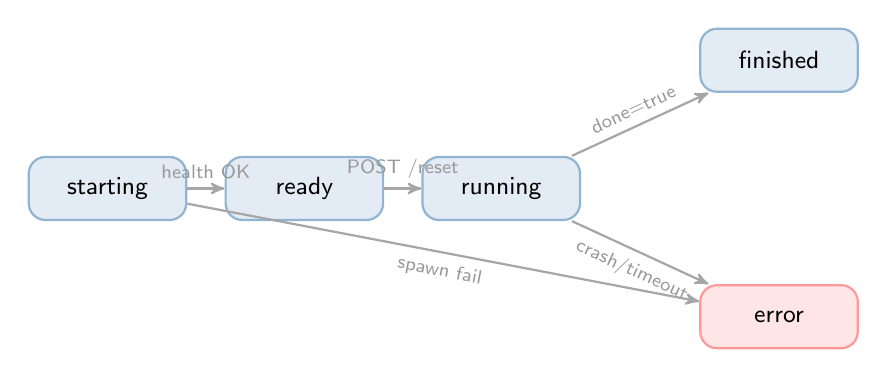
\begin{tikzpicture}[node distance=2.5cm, >=stealth',
    state/.style={draw, rounded corners=6pt, minimum width=2cm,
                  minimum height=0.8cm, font=\small\sffamily,
                  fill=orchcolor!15, draw=orchcolor!60, thick}]
  \node[state] (starting) {starting};
  \node[state, right of=starting] (ready) {ready};
  \node[state, right of=ready] (running) {running};
  \node[state, above right=0.8cm and 1.5cm of running] (finished) {finished};
  \node[state, below right=0.8cm and 1.5cm of running, fill=red!10, draw=red!40]
    (error) {error};

  \draw[arrow] (starting) -- node[label, above] {health OK} (ready);
  \draw[arrow] (ready) -- node[label, above] {POST /reset} (running);
  \draw[arrow] (running) -- node[label, above, sloped] {done=true} (finished);
  \draw[arrow] (running) -- node[label, below, sloped] {crash/timeout} (error);
  \draw[arrow] (starting) -- node[label, below, sloped] {spawn fail} (error);
\end{tikzpicture}
\caption{États d'une session}
\label{fig:session-lifecycle}
\end{figure}

\subsection{Timeout d'inactivité}

Chaque requête proxy appelle \code{touch\_session()} qui met à jour
\code{last\_activity}. Un task asyncio vérifie toutes les 30\,s si une
session est inactive depuis plus de 3\,minutes (\code{\_IDLE\_TIMEOUT = 180}).
Les sessions inactives sont détruites automatiquement (processus tué, port
libéré).

% ======================================================================
\section{Architecture des modules (bas niveau)}
\label{sec:archi-bas}
% ======================================================================

\subsection{Hiérarchie des packages}

\begin{figure}[H]
\centering
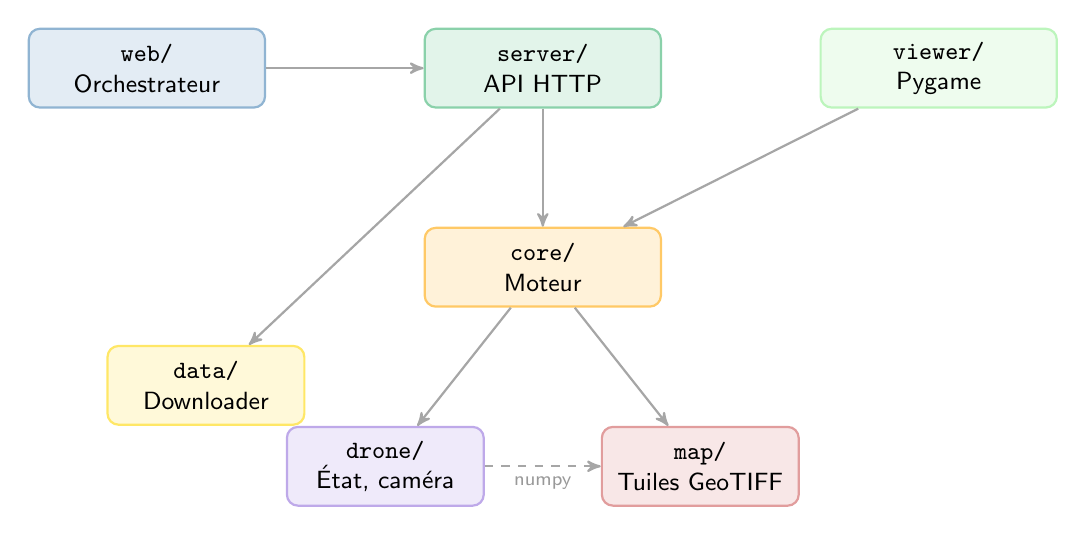
\begin{tikzpicture}[node distance=1cm and 1.5cm]

  \node[component=orchcolor, minimum width=3cm]
    (web) {\code{web/}\\Orchestrateur};
  \node[component=simcolor, minimum width=3cm, right=2cm of web]
    (server) {\code{server/}\\API HTTP};
  \node[component=viewercolor, minimum width=3cm, right=2cm of server]
    (vw) {\code{viewer/}\\Pygame};

  \node[component=corecolor, minimum width=3cm, below=1.5cm of server]
    (core) {\code{core/}\\Moteur};

  \node[component=dronecolor, minimum width=2.5cm, below=1.5cm of core,
        xshift=-2cm]
    (drone) {\code{drone/}\\État, caméra};
  \node[component=mapcolor, minimum width=2.5cm, below=1.5cm of core,
        xshift=2cm]
    (map) {\code{map/}\\Tuiles GeoTIFF};

  \node[component=datacolor, minimum width=2.5cm, left=1.5cm of core,
        yshift=-1.5cm]
    (dl) {\code{data/}\\Downloader};

  % --- Dependencies ---
  \draw[arrow] (web) -- (server);
  \draw[arrow] (server) -- (core);
  \draw[arrow] (vw) -- (core);
  \draw[arrow] (core) -- (drone);
  \draw[arrow] (core) -- (map);
  \draw[arrow] (server) -- (dl);
  \draw[arrow, dashed] (drone) -- node[label, below] {numpy} (map);

\end{tikzpicture}
\caption{Dépendances entre packages --- flux descendant strict, aucune
         dépendance circulaire}
\label{fig:packages}
\end{figure}

\subsection{Module \code{map/} --- Gestion géospatiale}

\begin{table}[H]
\centering\small
\begin{tabular}{llp{7.5cm}}
\toprule
\textbf{Classe} & \textbf{Fichier} & \textbf{Rôle} \\
\midrule
\code{Modality}      & \code{modality.py}     & Enum des 10 modalités FLAIR-HUB avec
                                                  \code{ModalitySpec} \\
\code{MapBounds}     & \code{map\_manager.py} & Rectangle englobant avec intersections \\
\code{MapManager}    & \code{map\_manager.py} & Moteur spatial~: découverte de tuiles,
                                                  grille, extraction de régions \\
\code{TileInfo}      & \code{tile\_loader.py} & Métadonnées d'une tuile (path, bounds) \\
\code{TileData}      & \code{tile\_loader.py} & Tuile chargée~: data array + bounds \\
\bottomrule
\end{tabular}
\caption{Classes du module \code{map/}}
\end{table}

Fonctions clés~:
\begin{itemize}
  \item \code{discover\_modalities(parent, domain)}~: scanne les répertoires
        frères pour trouver toutes les modalités disponibles.
  \item \code{MapManager.get\_region(x, y, half, size)}~: extrait et assemble
        les tuiles en une image continue redimensionnée via PIL LANCZOS.
  \item Système de coordonnées~: EPSG:2154 (Lambert-93, mètres).
\end{itemize}

\subsection{Module \code{drone/} --- État du drone et capteurs}

\begin{table}[H]
\centering\small
\begin{tabular}{llp{7.5cm}}
\toprule
\textbf{Classe} & \textbf{Fichier} & \textbf{Rôle} \\
\midrule
\code{DroneConfig}     & \code{drone.py}     & Limites physiques~: $z_{\min}$, $z_{\max}$,
                                                 distance max \\
\code{DroneState}      & \code{drone.py}     & Position courante $(x,y,z)$, heading,
                                                 compteurs \\
\code{Drone}           & \code{drone.py}     & reset, move (avec clampage aux bornes) \\
\code{CameraConfig}    & \code{camera.py}    & FOV (90°), taille image (500\,px) \\
\code{CameraModel}     & \code{camera.py}    & Géométrie nadir, capture d'image \\
\code{TelemetryRecord} & \code{telemetry.py} & Snapshot gelé par pas de temps \\
\code{FlightLog}       & \code{telemetry.py} & Journal de vol complet \\
\bottomrule
\end{tabular}
\caption{Classes du module \code{drone/}}
\end{table}

\subsubsection{Modèle de caméra}

La caméra pointe toujours au nadir.  La couverture au sol dépend de
l'altitude~:

\begin{equation}
  \text{empreinte} = 2 \times z \times \tan\!\left(\frac{\text{FOV}}{2}\right)
  \qquad\qquad
  \text{GSD} = \frac{\text{empreinte}}{\text{image\_size}}
\end{equation}

\begin{table}[H]
\centering\small
\begin{tabular}{rrr}
\toprule
\textbf{Altitude (m)} & \textbf{Empreinte (m)} & \textbf{GSD (m/px)} \\
\midrule
10  & 20   & 0.04 \\
50  & 100  & 0.20 \\
100 & 200  & 0.40 \\
200 & 400  & 0.80 \\
500 & 1000 & 2.00 \\
\bottomrule
\end{tabular}
\caption{Couverture au sol (FOV = 90°, image\_size = 500\,px)}
\end{table}

\subsection{Module \code{core/} --- Moteur de simulation}

\begin{table}[H]
\centering\small
\begin{tabular}{llp{7.5cm}}
\toprule
\textbf{Classe} & \textbf{Fichier} & \textbf{Rôle} \\
\midrule
\code{ActionType}      & \code{action.py}      & Enum~: MOVE, FOUND, STOP \\
\code{Action}          & \code{action.py}      & Commande gelée~: $(dx, dy, dz, type)$ \\
\code{Observation}     & \code{observation.py}  & Image + état + done + result \\
\code{EpisodeResult}   & \code{observation.py}  & success, reason, steps, distance \\
\code{FlairSimulator}  & \code{simulator.py}    & Classe principale du simulateur \\
\code{SimulatorConfig} & \code{simulator.py}    & Configuration globale \\
\code{Scenario}        & \code{scenario.py}     & Mission YAML complète \\
\code{ScenarioLoader}  & \code{scenario.py}     & Chargement et cache des scénarios \\
\code{GridOverlay}     & \code{grid.py}         & Grille $N{\times}N$ pour prompting VLM \\
\bottomrule
\end{tabular}
\caption{Classes du module \code{core/}}
\end{table}

Conditions de fin d'épisode~:
\begin{enumerate}
  \item \textbf{FOUND}~: l'agent déclare la cible trouvée. \code{success}
        dépend de la distance au target (si scénario actif).
  \item \textbf{STOP}~: arrêt volontaire (\code{success=False}).
  \item \textbf{Limite de pas}~: \code{max\_steps} atteint
        (\code{success=False}).
\end{enumerate}

\subsection{Module \code{server/} --- API HTTP REST}

Serveur FastAPI créé par la factory \code{create\_app()}.  Un seul
processus sert une seule simulation.  Voir section~\ref{sec:api-sim}
pour la référence complète des endpoints.

\subsection{Module \code{web/} --- Orchestrateur web}

\begin{table}[H]
\centering\small
\begin{tabular}{llp{7.5cm}}
\toprule
\textbf{Fichier} & \textbf{Classe} & \textbf{Rôle} \\
\midrule
\code{app.py}         & ---                & FastAPI app~: routes, proxy, middleware \\
\code{sessions.py}    & \code{SessionManager} & Spawn/destroy subprocess, pool de ports,
                                                 health check, idle timeout \\
\code{leaderboard.py} & \code{Leaderboard}    & SQLite CRUD~: submit, query, ranking \\
\code{cli.py}         & ---                & Parsing CLI \\
\code{static/}        & ---                & SPA vanilla JS (HTML + CSS + JS) \\
\bottomrule
\end{tabular}
\caption{Fichiers du module \code{web/}}
\end{table}

\subsection{Module \code{viewer/} --- Visualisation Pygame}

Trois modes de fonctionnement~:

\begin{table}[H]
\centering\small
\begin{tabular}{llp{7.5cm}}
\toprule
\textbf{Mode} & \textbf{Flag} & \textbf{Description} \\
\midrule
local   & \code{--mode local}   & Simulateur local, vol direct au clavier \\
observe & \code{--mode observe} & Connexion SSE au serveur, lecture seule \\
fly     & \code{--mode fly}     & Connexion HTTP, envoi de \code{POST /step} \\
\bottomrule
\end{tabular}
\caption{Modes du viewer}
\end{table}

\subsection{Module \code{data/} --- Téléchargement automatique}

\code{HubDownloader} télécharge les données depuis HuggingFace
(\code{IGNF/FLAIR-HUB}).  Workflow~: \code{hf\_hub\_download()} $\to$
\code{zipfile.extractall()} $\to$ suppression du ZIP.
Nettoyage automatique (\code{shutil.rmtree}) à l'arrêt du serveur.

% ======================================================================
\section{Architecture du front-end SPA}
\label{sec:archi-spa}
% ======================================================================

\begin{figure}[H]
\centering
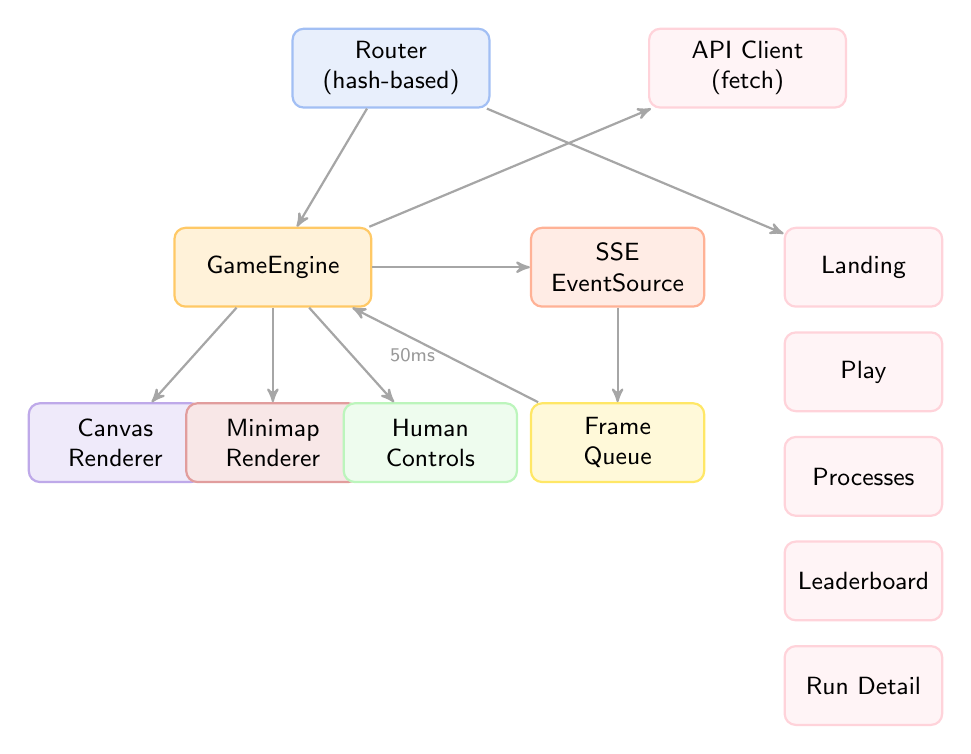
\begin{tikzpicture}[node distance=0.8cm and 1.5cm]

  \node[component=webcolor, minimum width=2.5cm]
    (router) {Router\\(hash-based)};
  \node[component=clientcolor, minimum width=2.5cm, right=2cm of router]
    (api) {API Client\\(fetch)};

  \node[component=corecolor, minimum width=2.5cm, below=1.5cm of router,
        xshift=-1.5cm]
    (engine) {GameEngine};
  \node[component=dronecolor, minimum width=2.2cm, below=1.2cm of engine,
        xshift=-2cm]
    (canvas) {Canvas\\Renderer};
  \node[component=mapcolor, minimum width=2.2cm, below=1.2cm of engine]
    (minimap) {Minimap\\Renderer};
  \node[component=viewercolor, minimum width=2.2cm, below=1.2cm of engine,
        xshift=2cm]
    (controls) {Human\\Controls};

  \node[component=ssecolor, minimum width=2.2cm, right=2cm of engine]
    (sse) {SSE\\EventSource};
  \node[component=datacolor, minimum width=2.2cm, below=1.2cm of sse]
    (queue) {Frame\\Queue};

  % Vues
  \node[component=clientcolor, minimum width=2cm, below=1.5cm of router,
        xshift=6cm]
    (v1) {Landing};
  \node[component=clientcolor, minimum width=2cm, below=0.3cm of v1]
    (v2) {Play};
  \node[component=clientcolor, minimum width=2cm, below=0.3cm of v2]
    (v3) {Processes};
  \node[component=clientcolor, minimum width=2cm, below=0.3cm of v3]
    (v4) {Leaderboard};
  \node[component=clientcolor, minimum width=2cm, below=0.3cm of v4]
    (v5) {Run Detail};

  \draw[arrow] (router) -- (engine);
  \draw[arrow] (engine) -- (canvas);
  \draw[arrow] (engine) -- (minimap);
  \draw[arrow] (engine) -- (controls);
  \draw[arrow] (engine) -- (sse);
  \draw[arrow] (sse) -- (queue);
  \draw[arrow] (queue) -- node[label, left] {50ms} (engine);
  \draw[arrow] (engine) -- (api);
  \draw[arrow] (router) -- (v1);

\end{tikzpicture}
\caption{Architecture du front-end SPA (vanilla JS, 1648 lignes)}
\label{fig:spa-archi}
\end{figure}

\textbf{Classes principales~:}
\begin{itemize}
  \item \code{GameEngine}~: gère le cycle de jeu, la connexion SSE,
        le rendu frame-by-frame, la détection de fin d'épisode.
  \item \code{CanvasRenderer}~: dessine l'image cockpit (700$\times$700)
        avec un réticule central.
  \item \code{MinimapRenderer}~: minimap 180$\times$180 avec trajectoire,
        drone, cible.
  \item \code{HumanControls}~: AZERTY/QWERTY, slider de pas, debounce.
\end{itemize}

\textbf{Mécanisme de rendu fluide~:}
\begin{enumerate}
  \item Le serveur décompose un mouvement en micro-pas ($\sim$10\,m).
  \item Chaque micro-pas est diffusé via SSE avec 50\,ms de délai.
  \item Le JS empile les frames dans \code{\_frameQueue[]}.
  \item Un timer à 50\,ms dépile une frame à la fois ($\sim$20 FPS).
  \item L'input utilisateur est bloqué (\code{\_processing=true})
        jusqu'à la réception du pas logique final.
\end{enumerate}

% ======================================================================
\section{API du serveur simulateur}
\label{sec:api-sim}
% ======================================================================

Tous les endpoints sont servis par un unique processus simulateur.
L'URL de base est \code{http://127.0.0.1:8000} en mode standalone,
ou \code{http://127.0.0.1:\{port\}} en mode sous-processus.

\subsection{\apiendpoint{POST}{/reset} --- Démarrer un épisode}

\begin{table}[H]
\centering\small
\begin{tabular}{lp{10cm}}
\toprule
\textbf{Champ} & \textbf{Détail} \\
\midrule
Query params & \code{?grid=N} (int, optionnel) --- taille de la grille overlay \\
\midrule
Request body & \code{ResetRequest} (optionnel) \\
& \code{x}: float$|$null --- position de départ est \\
& \code{y}: float$|$null --- position de départ nord \\
& \code{z}: float$|$null --- altitude de départ \\
& \code{scenario\_id}: string$|$null --- scénario à charger \\
\midrule
Response & \code{ObservationResponse} (voir section~\ref{sec:obs-format}) \\
Erreurs & 400 (scénarios non configurés), 404 (scénario introuvable) \\
Effets & Broadcast SSE à tous les abonnés \\
\bottomrule
\end{tabular}
\end{table}

\subsection{\apiendpoint{POST}{/step} --- Envoyer une action}

\begin{table}[H]
\centering\small
\begin{tabular}{lp{10cm}}
\toprule
\textbf{Champ} & \textbf{Détail} \\
\midrule
Query params & \code{?grid=N} (int, optionnel) \\
\midrule
Request body & \code{StepRequest} \\
& \code{dx}: float (défaut 0.0) --- déplacement est \\
& \code{dy}: float (défaut 0.0) --- déplacement nord \\
& \code{dz}: float (défaut 0.0) --- déplacement altitude \\
& \code{action\_type}: \code{"move"}$|$\code{"found"}$|$\code{"stop"} \\
& \code{reason}: string$|$null --- raisonnement de l'agent \\
\midrule
Response & \code{ObservationResponse} \\
Erreurs & 409 (pas d'épisode actif), 422 (type d'action invalide) \\
\midrule
Smooth step & Si \code{smooth\_step\_size > 0} et distance $>$ seuil~:\\
& décomposition en $N$ micro-pas, broadcast SSE intermédiaire\\
& avec \code{asyncio.sleep(0.05)}.  Compteur de pas~: +1 seul.\\
\bottomrule
\end{tabular}
\end{table}

\subsection{\apiendpoint{GET}{/state} --- État courant du drone}

\begin{table}[H]
\centering\small
\begin{tabular}{lp{10cm}}
\toprule
Response & \code{DroneStateResponse}: \code{\{x, y, z, heading, step\_count,
          total\_distance\}} \\
Erreurs & 409 (pas d'épisode actif) \\
\bottomrule
\end{tabular}
\end{table}

\subsection{\apiendpoint{GET}{/snapshot} --- Dernière observation cachée}

\begin{table}[H]
\centering\small
\begin{tabular}{lp{10cm}}
\toprule
Purpose & Retourne la dernière \code{ObservationResponse} en cache. Utile pour les
          spectateurs rejoignant en cours de session. \\
Response & JSON brut de la dernière observation \\
Erreurs & 404 (aucune observation encore émise) \\
\bottomrule
\end{tabular}
\end{table}

\subsection{\apiendpoint{GET}{/telemetry} --- Journal de vol}

\begin{table}[H]
\centering\small
\begin{tabular}{lp{10cm}}
\toprule
Response & \code{TelemetryResponse}~: \\
& \code{total\_steps}, \code{total\_distance}, \code{clips\_count},
  \code{altitude\_range} \\
& \code{records[]}: \code{\{step, x, y, z, dx, dy, dz,
  ground\_footprint, was\_clipped, reason\}} \\
\bottomrule
\end{tabular}
\end{table}

\subsection{\apiendpoint{GET}{/config} --- Configuration du simulateur}

\begin{table}[H]
\centering\small
\begin{tabular}{lp{10cm}}
\toprule
Response & \code{ConfigResponse}~: \\
& \code{data\_dir}, \code{roi}, \code{n\_tiles}, \code{pixel\_size\_m},
  \code{tile\_ground\_size} \\
& \code{map\_bounds}: \code{\{x\_min, y\_min, x\_max, y\_max, width, height\}} \\
& \code{drone}: \code{\{z\_min, z\_max, default\_altitude, max\_step\_distance\}} \\
& \code{camera}: \code{\{fov\_deg, image\_size\}} \\
& \code{max\_steps}, \code{is\_running}, \code{scenario\_id} \\
\bottomrule
\end{tabular}
\end{table}

\subsection{\apiendpoint{GET}{/scenarios} --- Liste des scénarios}

\begin{table}[H]
\centering\small
\begin{tabular}{lp{10cm}}
\toprule
Response & \code{ScenariosListResponse}: \\
& \code{scenarios[]}: \code{\{scenario\_id, name, description, max\_steps,
  target\_radius, environment[], difficulty\}} \\
\bottomrule
\end{tabular}
\end{table}

\subsection{\apiendpoint{GET}{/overview} --- Image vue d'ensemble}

\begin{table}[H]
\centering\small
\begin{tabular}{lp{10cm}}
\toprule
Query params & \code{?size=1024} (int) --- taille de l'image en pixels \\
Response & JPEG binaire avec headers personnalisés~:\\
& \code{X-Bounds-Xmin}, \code{X-Bounds-Ymin}, \code{X-Bounds-Xmax},
  \code{X-Bounds-Ymax} \\
Note & Image cachée après la première génération \\
\bottomrule
\end{tabular}
\end{table}

\subsection{\apiendpoint{GET}{/events} --- Flux SSE}
\label{sec:sse}

\begin{table}[H]
\centering\small
\begin{tabular}{lp{10cm}}
\toprule
Response & \code{text/event-stream} \\
Événements & \code{event: observation} + \code{data: <ObservationResponse JSON>} \\
Keep-alive & Commentaire \code{:keep-alive} toutes les 30\,s \\
Init & Commentaire \code{:connected} immédiat (flush des en-têtes) \\
Queue & \code{asyncio.Queue(maxsize=64)} par abonné. Si pleine, l'événement
        le plus ancien est supprimé \\
\bottomrule
\end{tabular}
\end{table}

\subsection{Format \code{ObservationResponse}}
\label{sec:obs-format}

\begin{lstlisting}[style=json, caption={Structure complète d'une ObservationResponse}]
{
  "step": 42,
  "done": false,
  "drone_state": {
    "x": 923456.2, "y": 6345123.8, "z": 100.0,
    "heading": 0.0, "step_count": 42,
    "total_distance": 523.4
  },
  "ground_footprint": 200.0,
  "ground_resolution": 0.4,
  "image_base64": "<PNG en base64>",
  "image_width": 500,
  "image_height": 500,
  "result": null,
  "metadata": {
    "roi": "UU-S2-1",
    "primary_modality": "AERIAL_RGBI",
    "distance_to_target": "42.5"
  },
  "images": {
    "AERIAL_RGBI": "<base64 PNG>",
    "DEM_ELEV": "<base64 PNG>"
  }
}
\end{lstlisting}

Lorsque \code{done=true}, le champ \code{result} contient~:
\begin{lstlisting}[style=json]
{
  "success": true,
  "reason": "Agent declared FOUND within 42.5 m of target",
  "steps_taken": 42,
  "distance_travelled": 523.4
}
\end{lstlisting}

% ======================================================================
\section{API de l'orchestrateur web}
\label{sec:api-orch}
% ======================================================================

Tous les endpoints sont préfixés par \code{/api/} sauf la redirection
racine et les fichiers statiques.

\subsection{\apiendpoint{GET}{/} --- Redirection vers la SPA}

Redirection 302 vers \code{/static/index.html}.

\subsection{\apiendpoint{GET}{/api/status} --- Health check}

\begin{lstlisting}[style=json]
{ "status": "ok", "active_sessions": 3, "scenarios_dir": "scenarios/" }
\end{lstlisting}

\subsection{\apiendpoint{GET}{/api/scenarios} --- Liste des scénarios}

Retourne tous les scénarios avec détails complets (dataset, start, target,
prompt, environment, difficulty).

\subsection{\apiendpoint{GET}{/api/scenarios/\{id\}} --- Détail d'un scénario}

Retourne un scénario avec ses templates de prompt pour les agents VLM.

\subsection{\apiendpoint{GET}{/api/scenarios/\{id\}/overview} --- Image overview}

Retourne l'image JPEG de vue d'ensemble pré-générée avec headers
\code{X-Bounds-*}.

\subsection{\apiendpoint{POST}{/api/sessions} --- Créer une session}

\begin{table}[H]
\centering\small
\begin{tabular}{lp{10cm}}
\toprule
Request body & \\
& \code{scenario\_id}: string (requis) \\
& \code{mode}: \code{"human"} (défaut) $|$ \code{"ai"} \\
& \code{player\_name}: string$|$null \\
& \code{model\_info}: object$|$null --- métadonnées du modèle AI \\
\midrule
Auth & Mode AI~: header \code{Authorization: Bearer <FLAIRSIM\_API\_KEY>} requis \\
& Mode human~: aucune authentification \\
\midrule
Response & \code{\{session\_id, scenario\_id, mode, port, status: "ready",
          created\_at, base\_url\}} \\
Erreurs & 400 (champs manquants), 401 (clé API invalide), 404 (scénario
          introuvable), 500 (échec spawn) \\
\midrule
Effets & Spawn un sous-processus \code{python -m flairsim.server}, health
         check GET /config pendant 30\,s max \\
\bottomrule
\end{tabular}
\end{table}

\subsection{\apiendpoint{GET}{/api/sessions} --- Lister les sessions}

Retourne \code{\{"sessions": [...]\}}.

\subsection{\apiendpoint{GET}{/api/sessions/\{id\}} --- État d'une session}

Vérifie aussi si le sous-processus est toujours vivant.

\subsection{\apiendpoint{DELETE}{/api/sessions/\{id\}} --- Détruire une session}

Tue le sous-processus, libère le port.

\subsection{\apiendpoint{ANY}{/api/sessions/\{id\}/sim/\{path\}} --- Proxy}

\begin{table}[H]
\centering\small
\begin{tabular}{lp{10cm}}
\toprule
Méthodes & GET, POST, PUT, DELETE, PATCH \\
Purpose & Relaye toute requête vers le sous-processus simulateur \\
SSE & Quand \code{path == "events"} et GET~: proxy SSE streaming via
      \code{httpx.AsyncClient.stream()} \\
Activité & Appelle \code{touch\_session()} à chaque requête \\
Erreurs & 404 (session introuvable), 502 (simulateur en erreur),
          503 (encore en démarrage), 504 (timeout) \\
\bottomrule
\end{tabular}
\end{table}

\subsection{\apiendpoint{GET}{/api/leaderboard} --- Classement}

\begin{table}[H]
\centering\small
\begin{tabular}{lp{10cm}}
\toprule
Query params & \code{?scenario\_id=...}, \code{?mode=human|ai},
               \code{?limit=50} \\
Tri & \code{ORDER BY success DESC, steps\_taken ASC,
      distance\_travelled ASC} \\
Response & \code{\{"runs": [...]\}} \\
\bottomrule
\end{tabular}
\end{table}

\subsection{\apiendpoint{POST}{/api/leaderboard} --- Soumettre un run}

\begin{table}[H]
\centering\small
\begin{tabular}{lp{10cm}}
\toprule
Request body & \code{scenario\_id} (requis), \code{mode} (requis) \\
& \code{player\_name}, \code{model\_name}, \code{success}, \code{reason} \\
& \code{steps\_taken}, \code{distance\_travelled}, \code{duration\_s} \\
& \code{trajectory}, \code{steps\_detail}, \code{model\_info}, \code{metrics},
  \code{score\_final} \\
Response & \code{\{"run\_id": "<UUID>"\}} \\
\bottomrule
\end{tabular}
\end{table}

\subsection{\apiendpoint{POST}{/api/leaderboard/submit} --- Alias}

Alias pour \code{POST /api/leaderboard}. Endpoint préféré pour les notebooks.

\subsection{\apiendpoint{GET}{/api/leaderboard/\{id\}} --- Détail d'un run}

Retourne l'objet complet avec colonnes JSON désérialisées.

% ======================================================================
\section{Leaderboard --- Schéma SQLite}
\label{sec:leaderboard}
% ======================================================================

\begin{lstlisting}[language=SQL, caption={Schéma de la table \code{runs}}]
CREATE TABLE IF NOT EXISTS runs (
  id                  TEXT PRIMARY KEY,  -- UUID
  session_id          TEXT,
  scenario_id         TEXT NOT NULL,
  player_name         TEXT,
  model_name          TEXT,
  mode                TEXT NOT NULL CHECK (mode IN ('human','ai')),
  success             INTEGER NOT NULL DEFAULT 0,
  reason              TEXT,
  steps_taken         INTEGER,
  distance_travelled  REAL,
  duration_s          REAL,
  trajectory          TEXT,     -- JSON serialized
  steps_detail        TEXT,     -- JSON serialized
  model_info          TEXT,     -- JSON serialized
  metrics             TEXT,     -- JSON serialized
  score_final         REAL,
  created_at          TEXT NOT NULL  -- ISO 8601
);
CREATE INDEX IF NOT EXISTS idx_runs_scenario
  ON runs (scenario_id);
\end{lstlisting}

Configuration~: \code{journal\_mode=WAL}, \code{check\_same\_thread=False}.
Migration automatique pour ajouter les colonnes manquantes.

% ======================================================================
\section{Format des scénarios YAML}
\label{sec:scenarios}
% ======================================================================

\begin{lstlisting}[style=yaml, caption={Structure d'un scénario YAML}]
scenario_id: find_target_D006
name: Find target in Isere
description: Navigate to locate a ground target

dataset:
  data_dir: D006-2020_AERIAL_RGBI
  domain: D006-2020
  roi: UU-S2-1
  modalities:
    - AERIAL_RGBI
  source: auto        # local | huggingface | auto

start:
  x: 1018422.0
  y: 6278750.0
  z: 150.0

target:
  x: 1018300.0
  y: 6278200.0
  radius: 50.0        # metres

max_steps: 200
environment: [rural]
difficulty: 2          # 1-3

prompt:
  system: |
    You are a drone navigation agent...
  user_template: |
    Position: ({x}, {y}, {z}). Step {step}/{max_steps}.
\end{lstlisting}

Placeholders disponibles dans \code{user\_template}~: \code{\{x\}},
\code{\{y\}}, \code{\{z\}}, \code{\{step\}}, \code{\{max\_steps\}},
\code{\{steps\_remaining\}}, \code{\{distance\}}.

% ======================================================================
\section{Diagrammes de séquence}
\label{sec:sequences}
% ======================================================================

\subsection{Création d'une session humaine (navigateur)}

\begin{figure}[H]
\centering
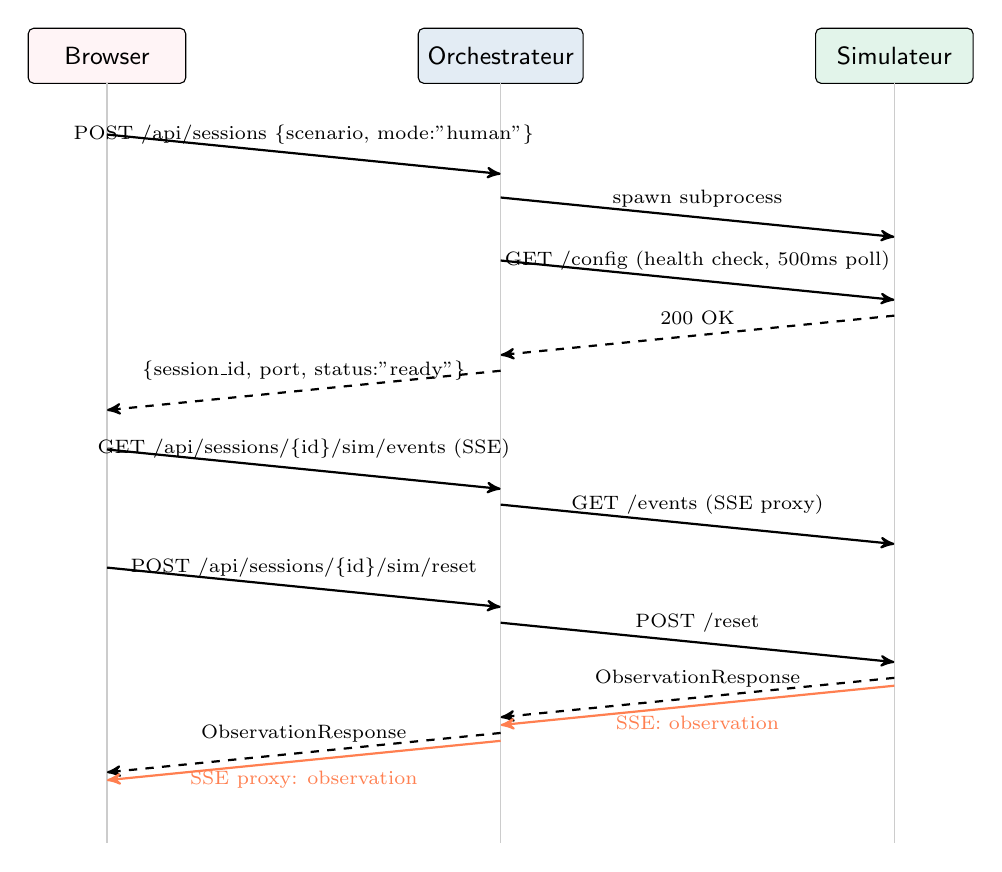
\begin{tikzpicture}[font=\small]
  % Actors
  \node[seqactor=clientcolor] (browser) at (0,0) {Browser};
  \node[seqactor=orchcolor]   (orch) at (5,0) {Orchestrateur};
  \node[seqactor=simcolor]    (sim) at (10,0) {Simulateur};

  % Lifelines
  \draw[gray!40] (0,-0.35) -- (0,-10);
  \draw[gray!40] (5,-0.35) -- (5,-10);
  \draw[gray!40] (10,-0.35) -- (10,-10);

  % Messages
  \draw[seqmsg] (0,-1) -- node[above, font=\scriptsize]
    {POST /api/sessions \{scenario, mode:"human"\}} (5,-1.5);

  \draw[seqmsg] (5,-1.8) -- node[above, font=\scriptsize]
    {spawn subprocess} (10,-2.3);

  \draw[seqmsg] (5,-2.6) -- node[above, font=\scriptsize]
    {GET /config (health check, 500ms poll)} (10,-3.1);

  \draw[seqret] (10,-3.3) -- node[above, font=\scriptsize]
    {200 OK} (5,-3.8);

  \draw[seqret] (5,-4) -- node[above, font=\scriptsize]
    {\{session\_id, port, status:"ready"\}} (0,-4.5);

  \draw[seqmsg] (0,-5) -- node[above, font=\scriptsize]
    {GET /api/sessions/\{id\}/sim/events (SSE)} (5,-5.5);

  \draw[seqmsg] (5,-5.7) -- node[above, font=\scriptsize]
    {GET /events (SSE proxy)} (10,-6.2);

  \draw[seqmsg] (0,-6.5) -- node[above, font=\scriptsize]
    {POST /api/sessions/\{id\}/sim/reset} (5,-7);

  \draw[seqmsg] (5,-7.2) -- node[above, font=\scriptsize]
    {POST /reset} (10,-7.7);

  \draw[seqret] (10,-7.9) -- node[above, font=\scriptsize]
    {ObservationResponse} (5,-8.4);

  \draw[seqret] (5,-8.6) -- node[above, font=\scriptsize]
    {ObservationResponse} (0,-9.1);

  % SSE push
  \draw[seqmsg, color=ssecolor] (10,-8) -- node[below, font=\scriptsize,
    color=ssecolor] {SSE: observation} (5,-8.5);
  \draw[seqmsg, color=ssecolor] (5,-8.7) -- node[below, font=\scriptsize,
    color=ssecolor] {SSE proxy: observation} (0,-9.2);

\end{tikzpicture}
\caption{Séquence~: création d'une session humaine}
\label{fig:seq-session}
\end{figure}

\subsection{Mouvement fluide (smooth step) via SSE}

\begin{figure}[H]
\centering
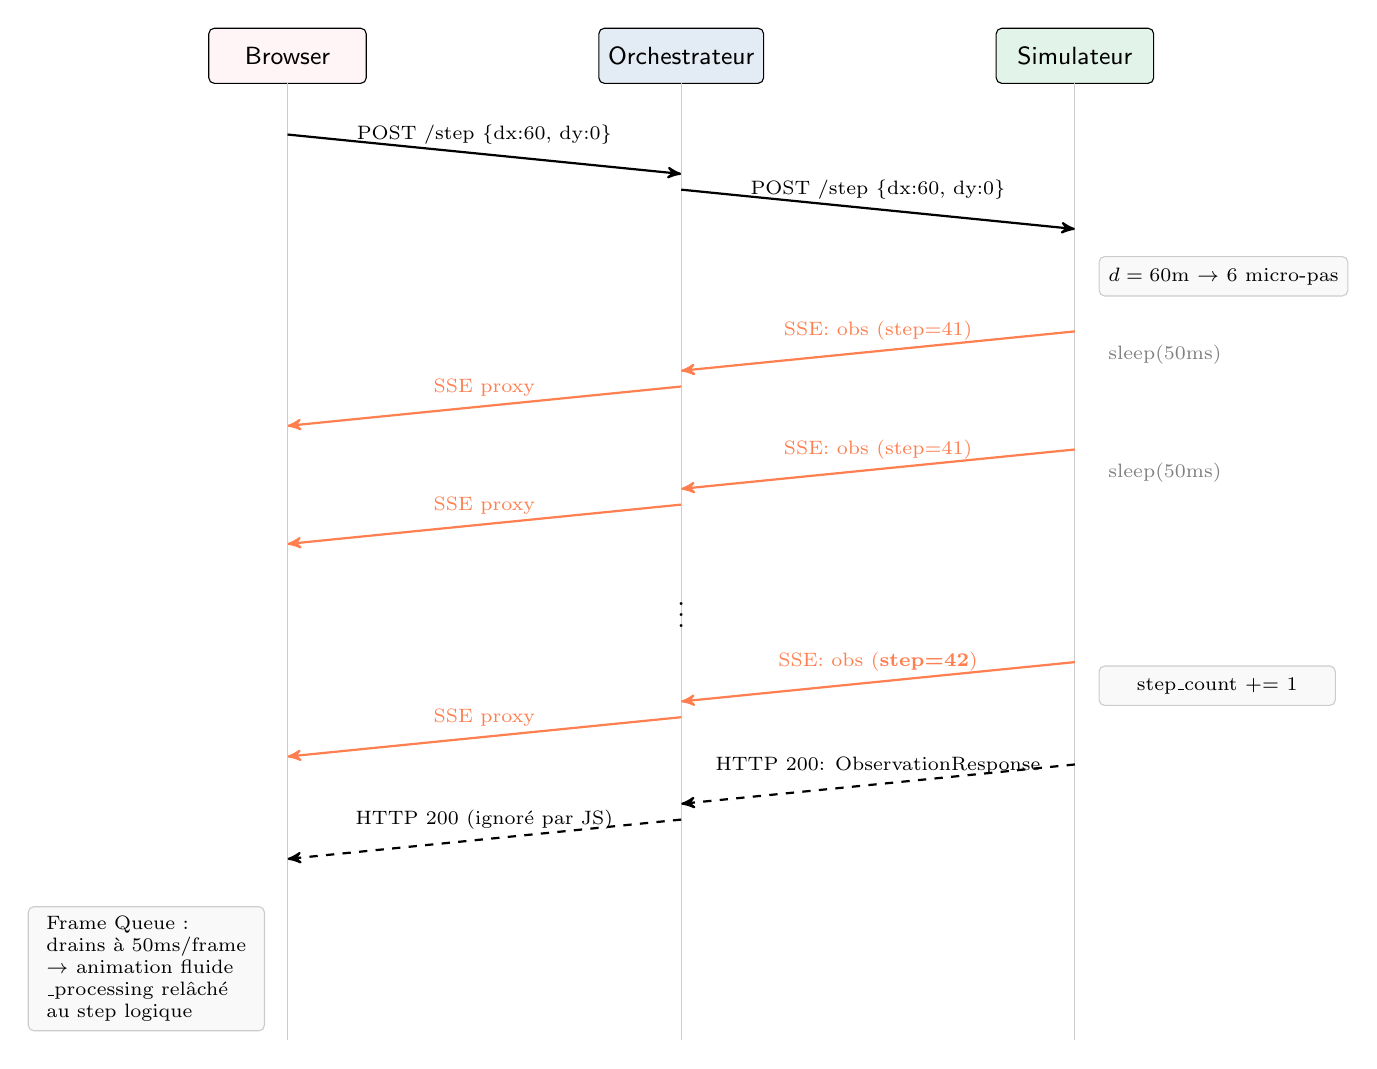
\begin{tikzpicture}[font=\small]
  % Actors
  \node[seqactor=clientcolor] (browser) at (0,0) {Browser};
  \node[seqactor=orchcolor]   (orch) at (5,0) {Orchestrateur};
  \node[seqactor=simcolor]    (sim) at (10,0) {Simulateur};

  % Lifelines
  \draw[gray!40] (0,-0.35) -- (0,-12.5);
  \draw[gray!40] (5,-0.35) -- (5,-12.5);
  \draw[gray!40] (10,-0.35) -- (10,-12.5);

  % Step request
  \draw[seqmsg] (0,-1) -- node[above, font=\scriptsize]
    {POST /step \{dx:60, dy:0\}} (5,-1.5);
  \draw[seqmsg] (5,-1.7) -- node[above, font=\scriptsize]
    {POST /step \{dx:60, dy:0\}} (10,-2.2);

  % Server decomposes: 60m / 10m = 6 micro-steps
  \node[seqbox, minimum width=3cm, minimum height=0.5cm, anchor=west,
        font=\scriptsize] at (10.3,-2.8)
    {$d=60$m $\to$ 6 micro-pas};

  % Micro-step 1
  \draw[seqmsg, color=ssecolor] (10,-3.5) -- node[above, font=\scriptsize,
    color=ssecolor] {SSE: obs (step=41)} (5,-4);
  \draw[seqmsg, color=ssecolor] (5,-4.2) -- node[above, font=\scriptsize,
    color=ssecolor] {SSE proxy} (0,-4.7);

  \node[font=\scriptsize, color=gray, anchor=west] at (10.3,-3.8)
    {sleep(50ms)};

  % Micro-step 2
  \draw[seqmsg, color=ssecolor] (10,-5) -- node[above, font=\scriptsize,
    color=ssecolor] {SSE: obs (step=41)} (5,-5.5);
  \draw[seqmsg, color=ssecolor] (5,-5.7) -- node[above, font=\scriptsize,
    color=ssecolor] {SSE proxy} (0,-6.2);

  \node[font=\scriptsize, color=gray, anchor=west] at (10.3,-5.3)
    {sleep(50ms)};

  % Dots
  \node[font=\normalsize] at (5,-7) {$\vdots$};

  % Final micro-step
  \draw[seqmsg, color=ssecolor] (10,-7.7) -- node[above, font=\scriptsize,
    color=ssecolor] {SSE: obs (\textbf{step=42})} (5,-8.2);
  \draw[seqmsg, color=ssecolor] (5,-8.4) -- node[above, font=\scriptsize,
    color=ssecolor] {SSE proxy} (0,-8.9);

  \node[seqbox, minimum width=3cm, minimum height=0.5cm, anchor=west,
        font=\scriptsize] at (10.3,-8)
    {step\_count += 1};

  % HTTP response (final)
  \draw[seqret] (10,-9) -- node[above, font=\scriptsize]
    {HTTP 200: ObservationResponse} (5,-9.5);
  \draw[seqret] (5,-9.7) -- node[above, font=\scriptsize]
    {HTTP 200 (ignoré par JS)} (0,-10.2);

  % JS frame queue
  \node[seqbox, minimum width=3cm, minimum height=1.2cm, anchor=north west,
        font=\scriptsize, align=left] at (-3.3,-10.8)
    {Frame Queue~:\\drains à 50ms/frame\\$\to$ animation fluide\\
     \_processing relâché\\au step logique};

\end{tikzpicture}
\caption{Séquence~: mouvement fluide avec micro-pas SSE}
\label{fig:seq-smooth}
\end{figure}

\subsection{Session AI depuis un notebook}

\begin{figure}[H]
\centering
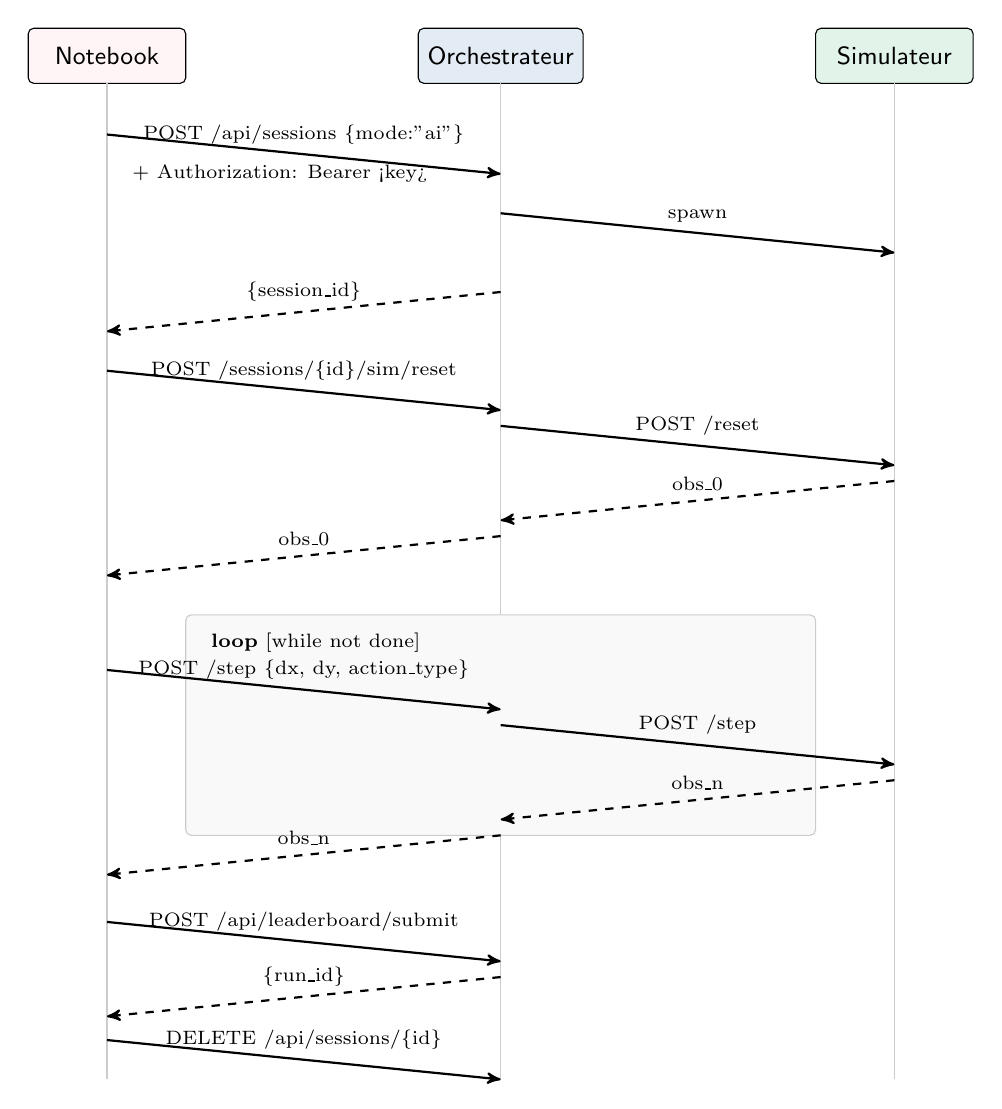
\begin{tikzpicture}[font=\small]
  % Actors
  \node[seqactor=clientcolor] (nb) at (0,0) {Notebook};
  \node[seqactor=orchcolor]   (orch) at (5,0) {Orchestrateur};
  \node[seqactor=simcolor]    (sim) at (10,0) {Simulateur};

  % Lifelines
  \draw[gray!40] (0,-0.35) -- (0,-13);
  \draw[gray!40] (5,-0.35) -- (5,-13);
  \draw[gray!40] (10,-0.35) -- (10,-13);

  % Create session
  \draw[seqmsg] (0,-1) -- node[above, font=\scriptsize]
    {POST /api/sessions \{mode:"ai"\}} (5,-1.5);
  \node[font=\scriptsize, anchor=west] at (0.2,-1.5)
    {+ Authorization: Bearer <key>};

  \draw[seqmsg] (5,-2) -- node[above, font=\scriptsize]
    {spawn} (10,-2.5);
  \draw[seqret] (5,-3) -- node[above, font=\scriptsize]
    {\{session\_id\}} (0,-3.5);

  % Reset
  \draw[seqmsg] (0,-4) -- node[above, font=\scriptsize]
    {POST /sessions/\{id\}/sim/reset} (5,-4.5);
  \draw[seqmsg] (5,-4.7) -- node[above, font=\scriptsize]
    {POST /reset} (10,-5.2);
  \draw[seqret] (10,-5.4) -- node[above, font=\scriptsize]
    {obs\_0} (5,-5.9);
  \draw[seqret] (5,-6.1) -- node[above, font=\scriptsize]
    {obs\_0} (0,-6.6);

  % Step loop
  \node[seqbox, minimum width=8cm, minimum height=2.8cm] at (5,-8.5) {};
  \node[font=\scriptsize, anchor=north west] at (1.2,-7.2)
    {\textbf{loop} [while not done]};

  \draw[seqmsg] (0,-7.8) -- node[above, font=\scriptsize]
    {POST /step \{dx, dy, action\_type\}} (5,-8.3);
  \draw[seqmsg] (5,-8.5) -- node[above, font=\scriptsize]
    {POST /step} (10,-9);
  \draw[seqret] (10,-9.2) -- node[above, font=\scriptsize]
    {obs\_n} (5,-9.7);
  \draw[seqret] (5,-9.9) -- node[above, font=\scriptsize]
    {obs\_n} (0,-10.4);

  % Leaderboard submit
  \draw[seqmsg] (0,-11) -- node[above, font=\scriptsize]
    {POST /api/leaderboard/submit} (5,-11.5);
  \draw[seqret] (5,-11.7) -- node[above, font=\scriptsize]
    {\{run\_id\}} (0,-12.2);

  % Cleanup
  \draw[seqmsg] (0,-12.5) -- node[above, font=\scriptsize]
    {DELETE /api/sessions/\{id\}} (5,-13);

\end{tikzpicture}
\caption{Séquence~: boucle complète d'un agent AI depuis un notebook}
\label{fig:seq-ai}
\end{figure}

\subsection{Spectateur rejoignant une session en cours}

\begin{figure}[H]
\centering
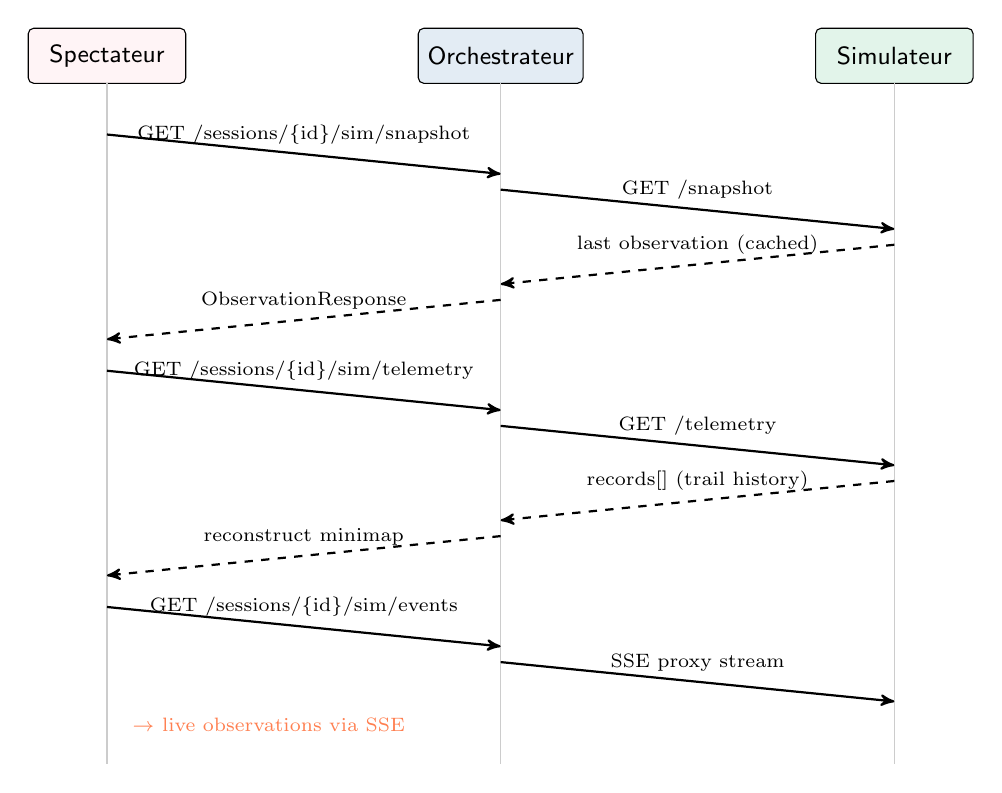
\begin{tikzpicture}[font=\small]
  % Actors
  \node[seqactor=clientcolor] (spec) at (0,0) {Spectateur};
  \node[seqactor=orchcolor]   (orch) at (5,0) {Orchestrateur};
  \node[seqactor=simcolor]    (sim) at (10,0) {Simulateur};

  % Lifelines
  \draw[gray!40] (0,-0.35) -- (0,-9);
  \draw[gray!40] (5,-0.35) -- (5,-9);
  \draw[gray!40] (10,-0.35) -- (10,-9);

  % Get snapshot
  \draw[seqmsg] (0,-1) -- node[above, font=\scriptsize]
    {GET /sessions/\{id\}/sim/snapshot} (5,-1.5);
  \draw[seqmsg] (5,-1.7) -- node[above, font=\scriptsize]
    {GET /snapshot} (10,-2.2);
  \draw[seqret] (10,-2.4) -- node[above, font=\scriptsize]
    {last observation (cached)} (5,-2.9);
  \draw[seqret] (5,-3.1) -- node[above, font=\scriptsize]
    {ObservationResponse} (0,-3.6);

  % Get telemetry
  \draw[seqmsg] (0,-4) -- node[above, font=\scriptsize]
    {GET /sessions/\{id\}/sim/telemetry} (5,-4.5);
  \draw[seqmsg] (5,-4.7) -- node[above, font=\scriptsize]
    {GET /telemetry} (10,-5.2);
  \draw[seqret] (10,-5.4) -- node[above, font=\scriptsize]
    {records[] (trail history)} (5,-5.9);
  \draw[seqret] (5,-6.1) -- node[above, font=\scriptsize]
    {reconstruct minimap} (0,-6.6);

  % Connect SSE
  \draw[seqmsg] (0,-7) -- node[above, font=\scriptsize]
    {GET /sessions/\{id\}/sim/events} (5,-7.5);
  \draw[seqmsg] (5,-7.7) -- node[above, font=\scriptsize]
    {SSE proxy stream} (10,-8.2);

  \node[font=\scriptsize, anchor=west, color=ssecolor] at (0.2,-8.5)
    {$\to$ live observations via SSE};

\end{tikzpicture}
\caption{Séquence~: spectateur rejoignant en cours de session}
\label{fig:seq-spectator}
\end{figure}

\subsection{Flux de données complet d'un pas de simulation}

\begin{figure}[H]
\centering
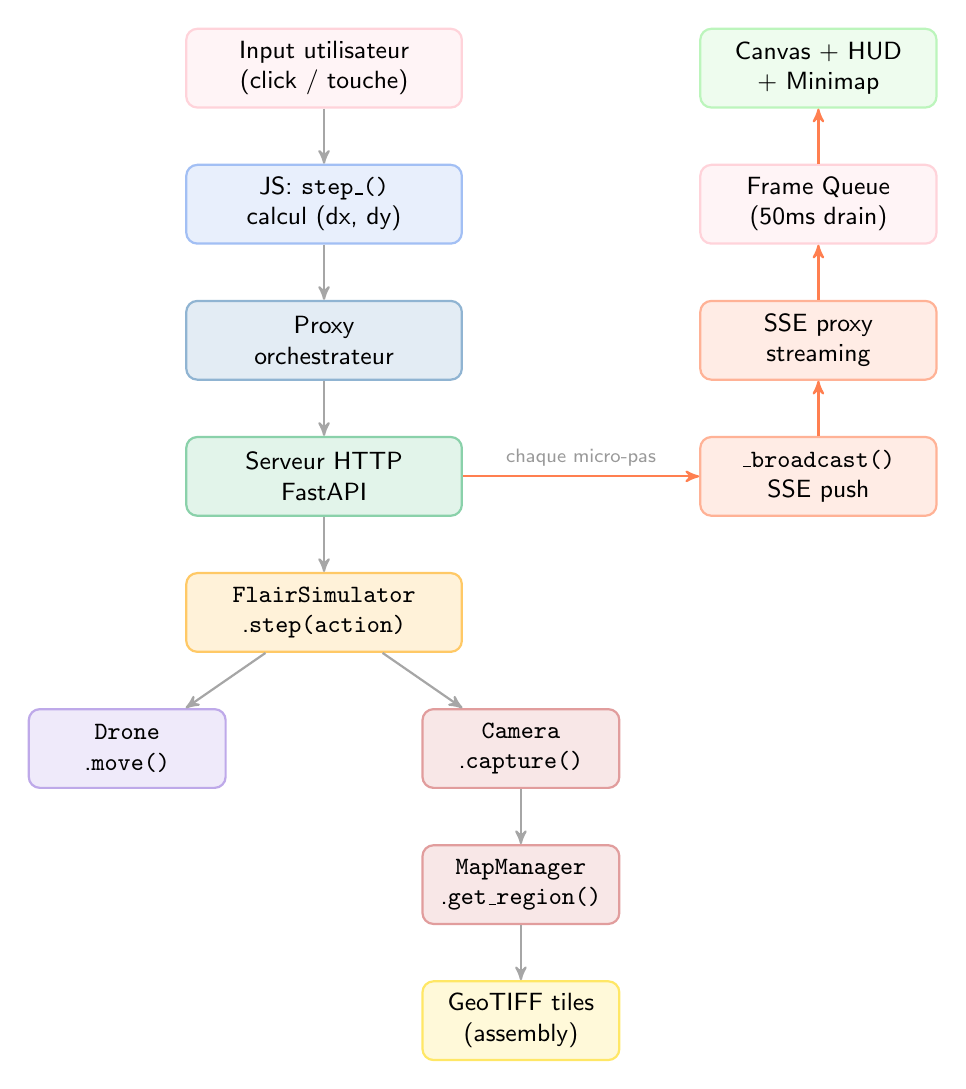
\begin{tikzpicture}[font=\small, node distance=0.7cm]

  \node[component=clientcolor, minimum width=3.5cm]
    (input) {Input utilisateur\\(click / touche)};

  \node[component=webcolor, minimum width=3.5cm, below=of input]
    (js) {JS: \code{step\_()}\\calcul (dx, dy)};

  \node[component=orchcolor, minimum width=3.5cm, below=of js]
    (proxy) {Proxy\\orchestrateur};

  \node[component=simcolor, minimum width=3.5cm, below=of proxy]
    (server) {Serveur HTTP\\FastAPI};

  \node[component=corecolor, minimum width=3.5cm, below=of server]
    (engine) {\code{FlairSimulator}\\.\code{step(action)}};

  \node[component=dronecolor, minimum width=2.5cm, below=of engine,
        xshift=-2.5cm]
    (drone) {\code{Drone}\\.\code{move()}};

  \node[component=mapcolor, minimum width=2.5cm, below=of engine,
        xshift=2.5cm]
    (camera) {\code{Camera}\\.\code{capture()}};

  \node[component=mapcolor, minimum width=2.5cm, below=of camera]
    (mapman) {\code{MapManager}\\.\code{get\_region()}};

  \node[component=datacolor, minimum width=2.5cm, below=of mapman]
    (tiles) {GeoTIFF tiles\\(assembly)};

  % Response path
  \node[component=ssecolor, minimum width=3cm, right=3cm of server]
    (broadcast) {\code{\_broadcast()}\\SSE push};

  \node[component=ssecolor, minimum width=3cm, above=of broadcast]
    (sseproxy) {SSE proxy\\streaming};

  \node[component=clientcolor, minimum width=3cm, above=of sseproxy]
    (frameq) {Frame Queue\\(50ms drain)};

  \node[component=viewercolor, minimum width=3cm, above=of frameq]
    (render) {Canvas + HUD\\+ Minimap};

  % Arrows down
  \draw[arrow] (input) -- (js);
  \draw[arrow] (js) -- (proxy);
  \draw[arrow] (proxy) -- (server);
  \draw[arrow] (server) -- (engine);
  \draw[arrow] (engine) -- (drone);
  \draw[arrow] (engine) -- (camera);
  \draw[arrow] (camera) -- (mapman);
  \draw[arrow] (mapman) -- (tiles);

  % Arrows right/up (SSE path)
  \draw[arrow, color=ssecolor] (server) -- node[label, above]
    {chaque micro-pas} (broadcast);
  \draw[arrow, color=ssecolor] (broadcast) -- (sseproxy);
  \draw[arrow, color=ssecolor] (sseproxy) -- (frameq);
  \draw[arrow, color=ssecolor] (frameq) -- (render);

\end{tikzpicture}
\caption{Flux de données complet~: de l'input utilisateur au rendu}
\label{fig:dataflow}
\end{figure}

% ======================================================================
\section{Authentification API}
\label{sec:auth}
% ======================================================================

\begin{enumerate}
  \item \textbf{Source de la clé}~: variable d'environnement
        \code{FLAIRSIM\_API\_KEY} ou fichier \code{.env} à la racine.
  \item \textbf{Portée}~: seul \code{POST /api/sessions} en mode
        \code{"ai"} exige la clé.
  \item \textbf{Header}~: \code{Authorization: Bearer <token>}.
  \item \textbf{Mode human}~: aucune authentification requise.
  \item \textbf{Sessions existantes}~: les requêtes proxy ne sont pas
        authentifiées (la session est déjà créée).
\end{enumerate}

Si aucune clé n'est configurée~: le serveur retourne 503 pour les
sessions AI (``AI API access not configured'').

% ======================================================================
\section{Données FLAIR-HUB}
\label{sec:data}
% ======================================================================

\subsection{Modalités supportées}

\begin{table}[H]
\centering\small
\begin{tabular}{llrrl}
\toprule
\textbf{Modalité} & \textbf{Suffixe} & \textbf{Résolution} & \textbf{Bandes}
  & \textbf{Type} \\
\midrule
AERIAL\_RGBI      & \code{AERIAL\_RGBI}      & 0.2\,m/px  & 4 & uint8 \\
AERIAL\_RLT\_PAN  & \code{AERIAL-RLT\_PAN}   & 0.4\,m/px  & 1 & uint8 \\
DEM\_ELEV         & \code{DEM\_ELEV}         & 0.2\,m/px  & 2 & float32 \\
SPOT\_RGBI        & \code{SPOT\_RGBI}        & 1.6\,m/px  & 4 & uint16 \\
SENTINEL1\_ASC    & \code{SENTINEL1-ASC\_TS} & 10.24\,m/px & 2 & float32 \\
SENTINEL1\_DESC   & \code{SENTINEL1-DESC\_TS}& 10.24\,m/px & 2 & float32 \\
SENTINEL2\_TS     & \code{SENTINEL2\_TS}     & 10.24\,m/px & 10 & uint16 \\
LABEL\_COSIA      & \code{AERIAL\_LABEL-COSIA} & 0.2\,m/px & 1 & uint8 \\
LABEL\_LPIS       & \code{ALL\_LABEL-LPIS}   & 0.2\,m/px  & 3 & uint8 \\
SENTINEL2\_MSK    & \code{SENTINEL2\_MSK-SC} & 10.24\,m/px & 2 & uint16 \\
\bottomrule
\end{tabular}
\caption{Modalités FLAIR-HUB (tous les patches couvrent
         $102.4\,\text{m} \times 102.4\,\text{m}$)}
\end{table}

\subsection{Téléchargement automatique}

Si \code{--domain D006-2020} est spécifié sans \code{--data-dir}~:
\begin{enumerate}
  \item \code{HubDownloader} télécharge depuis \code{IGNF/FLAIR-HUB}
        sur HuggingFace.
  \item Les ZIP sont extraits dans un répertoire temporaire.
  \item Nettoyage automatique à l'arrêt (SIGINT/SIGTERM).
\end{enumerate}

% ======================================================================
\section{Grille overlay pour VLMs}
\label{sec:grid}
% ======================================================================

La classe \code{GridOverlay} divise l'image en une grille $N \times N$
avec des labels alphanumériques (A1, A2, B1, ...), inspiré des
approches \textbf{Set-of-Mark}~\cite{som} et \textbf{Scaffold}~\cite{scaffold}.

Points d'intégration~:
\begin{itemize}
  \item API serveur~: \code{?grid=N} sur \code{/reset} et \code{/step}
  \item Viewer~: \code{--grid N} + touche G
  \item Programmatique~: \code{GridOverlay(n=4).draw(image)}
\end{itemize}

% ======================================================================
\section{Installation et utilisation}
\label{sec:usage}
% ======================================================================

\subsection{Installation}

\begin{lstlisting}[style=bash]
cd simulateur
uv sync --all-extras   # core + server + viewer + dev
\end{lstlisting}

\subsection{Lancer le simulateur (mode standalone)}

\begin{lstlisting}[style=bash]
# Donnees locales
uv run python -m flairsim.server --data-dir path/to/D004_AERIAL_RGBI

# Auto-download depuis HuggingFace
uv run python -m flairsim.server --domain D006-2020

# Avec scenario
uv run python -m flairsim.server \
    --data-root path/to/data --scenarios-dir scenarios/ \
    --scenario find_target_D006
\end{lstlisting}

\subsection{Lancer la plateforme web}

\begin{lstlisting}[style=bash]
uv run python -m flairsim.web \
    --scenarios-dir scenarios/ \
    --data-root path/to/data
\end{lstlisting}

Ouvrir \code{http://127.0.0.1:8080} dans le navigateur.

\subsection{Viewer Pygame}

\begin{lstlisting}[style=bash]
# Mode local
uv run python -m flairsim.viewer --data-dir path/to/data

# Mode observe (SSE)
uv run python -m flairsim.viewer --mode observe

# Mode fly (pilotage distant)
uv run python -m flairsim.viewer --mode fly
\end{lstlisting}

\subsection{Contrôles clavier}

\begin{table}[H]
\centering\small
\begin{tabular}{ll|ll}
\toprule
\textbf{Touche} & \textbf{Action} & \textbf{Touche} & \textbf{Action} \\
\midrule
Z / W / $\uparrow$ & Nord       & E        & Monter \\
S / $\downarrow$    & Sud        & A        & Descendre \\
D / $\rightarrow$   & Est        & +/--     & Taille du pas \\
Q / $\leftarrow$    & Ouest      & Espace   & FOUND \\
Tab                 & Modalité   & R        & Reset \\
H                   & HUD        & M        & Minimap \\
G                   & Grille     & Échap    & Quitter \\
\bottomrule
\end{tabular}
\caption{Contrôles clavier (web + viewer Pygame)}
\end{table}

% ======================================================================
\section{Tests}
\label{sec:tests}
% ======================================================================

La suite comprend \textbf{554 tests} couvrant tous les modules~:

\begin{lstlisting}[style=bash]
uv run pytest           # 554 tests, ~9s
uv run pytest -v        # verbeux
uv run pytest -x        # arret au premier echec
\end{lstlisting}

\begin{table}[H]
\centering\small
\begin{tabular}{lrl}
\toprule
\textbf{Fichier} & \textbf{Tests} & \textbf{Portée} \\
\midrule
\code{test\_action.py}         & 13 & Action, ActionType \\
\code{test\_camera.py}         & 15 & CameraModel \\
\code{test\_drone.py}          & 39 & Drone, DroneConfig \\
\code{test\_map\_manager.py}   & 44 & MapManager (GeoTIFFs synthétiques) \\
\code{test\_modality.py}       & 11 & Modality, ModalitySpec \\
\code{test\_multimodality.py}  & 12 & Multi-modality (intégration) \\
\code{test\_observation.py}    & 14 & Observation, EpisodeResult \\
\code{test\_scenario.py}       & 49 & Scenario, ScenarioLoader \\
\code{test\_server.py}         & 48 & Endpoints HTTP + SSE + Snapshot \\
\code{test\_simulator.py}      & 47 & FlairSimulator (intégration) \\
\code{test\_telemetry.py}      & 16 & TelemetryRecord, FlightLog \\
\code{test\_tile\_loader.py}   & 16 & TileInfo, TileData \\
\code{test\_downloader.py}     & 22 & HubDownloader (mock HF) \\
\code{test\_grid.py}           & 59 & GridOverlay \\
\code{test\_sessions.py}       & 52 & SessionManager (mock subprocess) \\
\code{test\_leaderboard.py}    & 30 & Leaderboard SQLite \\
\code{test\_web\_routes.py}    & 67 & Routes orchestrateur \\
\midrule
\textbf{Total}                 & \textbf{554} & \\
\bottomrule
\end{tabular}
\caption{Répartition des tests par fichier}
\end{table}

% ======================================================================
\section{Structure du projet}
\label{sec:structure}
% ======================================================================

\begin{lstlisting}[language={}, basicstyle=\ttfamily\scriptsize]
simulateur/
  flairsim/                  # Package principal
    __init__.py              # API publique (26 exports)
    data/                    # Telechargement HuggingFace
      downloader.py          # HubDownloader
    map/                     # Tuiles GeoTIFF, requetes spatiales
      modality.py            # Enum Modality (10 modalites)
      tile_loader.py         # TileInfo, TileData, read_tile()
      map_manager.py         # MapManager, MapBounds
    drone/                   # Etat du drone, camera, telemetrie
      drone.py               # Drone, DroneConfig, DroneState
      camera.py              # CameraModel, CameraConfig
      telemetry.py           # FlightLog, TelemetryRecord
    core/                    # Moteur de simulation
      action.py              # Action, ActionType (MOVE/FOUND/STOP)
      observation.py         # Observation, EpisodeResult
      simulator.py           # FlairSimulator, SimulatorConfig
      scenario.py            # Scenario, ScenarioLoader, ScenarioPrompt
      grid.py                # GridOverlay (SoM/Scaffold)
    server/                  # API HTTP REST + SSE (simulateur)
      app.py                 # FastAPI factory, 9 endpoints, SSE
      cli.py                 # CLI parsing, auto-download
    web/                     # Plateforme web (orchestrateur)
      app.py                 # FastAPI, routes, proxy, middleware
      sessions.py            # SessionManager (subprocess, ports)
      leaderboard.py         # SQLite CRUD, ranking, migration
      cli.py                 # CLI parsing
      static/                # SPA vanilla JS
        index.html           # 5 vues + modal resultats
        style.css            # Theme sombre, responsive (1188 lignes)
        app.js               # Router, GameEngine, Canvas, Minimap (1648 lignes)
    viewer/                  # Visualisation Pygame
      viewer.py              # FlairViewer (3 modes)
      remote.py              # ViewerObservation adapter
      minimap.py             # Minimap overlay
      hud.py                 # HUD overlay
  scenarios/                 # Fichiers YAML de scenarios
  tests/                     # 554 tests (17 fichiers)
  docs/                      # Documentation technique
  pyproject.toml             # Config package (hatchling)
\end{lstlisting}

% ======================================================================
\section{Références}
% ======================================================================

\begin{thebibliography}{9}

\bibitem{flairhub}
  Music, A. et al. (2025).
  \emph{FLAIR-HUB: A large-scale multimodal dataset for land-cover
  mapping.}
  arXiv:2506.07080.

\bibitem{flysearch}
  Majumdar, A. et al. (2025).
  \emph{FlySearch: A benchmark for evaluating VLM exploration
  capabilities with a UAV.}
  NeurIPS 2025. arXiv:2506.02896.

\bibitem{som}
  Yang, J. et al. (2023).
  \emph{Set-of-Mark prompting unleashes extraordinary visual grounding
  in GPT-4V.}
  arXiv:2310.11441.

\bibitem{scaffold}
  Lei, L. et al. (2024).
  \emph{Scaffolding coordinates to promote vision-language coordination
  in large multi-modal models.}
  arXiv:2402.12058.

\end{thebibliography}

\end{document}
